\documentclass{article}[18pt]
\ProvidesPackage{format}
%Page setup
\usepackage[utf8]{inputenc}
\usepackage[margin=0.7in]{geometry}
\usepackage{parselines} 
\usepackage[english]{babel}
\usepackage{fancyhdr}
\usepackage{titlesec}
\hyphenpenalty=10000

\pagestyle{fancy}
\fancyhf{}
\rhead{Sam Robbins}
\rfoot{Page \thepage}

%Characters
\usepackage{amsmath}
\usepackage{amssymb}
\usepackage{gensymb}
\newcommand{\R}{\mathbb{R}}

%Diagrams
\usepackage{pgfplots}
\usepackage{graphicx}
\usepackage{tabularx}
\usepackage{relsize}
\pgfplotsset{width=10cm,compat=1.9}
\usepackage{float}

%Length Setting
\titlespacing\section{0pt}{14pt plus 4pt minus 2pt}{0pt plus 2pt minus 2pt}
\newlength\tindent
\setlength{\tindent}{\parindent}
\setlength{\parindent}{0pt}
\renewcommand{\indent}{\hspace*{\tindent}}

%Programming Font
\usepackage{courier}
\usepackage{listings}
\usepackage{pxfonts}

%Lists
\usepackage{enumerate}
\usepackage{enumitem}

% Networks Macro
\usepackage{tikz}


% Commands for files converted using pandoc
\providecommand{\tightlist}{%
	\setlength{\itemsep}{0pt}\setlength{\parskip}{0pt}}
\usepackage{hyperref}

% Get nice commands for floor and ceil
\usepackage{mathtools}
\DeclarePairedDelimiter{\ceil}{\lceil}{\rceil}
\DeclarePairedDelimiter{\floor}{\lfloor}{\rfloor}

% Allow itemize to go up to 20 levels deep (just change the number if you need more you madman)
\usepackage{enumitem}
\setlistdepth{20}
\renewlist{itemize}{itemize}{20}

% initially, use dots for all levels
\setlist[itemize]{label=$\cdot$}

% customize the first 3 levels
\setlist[itemize,1]{label=\textbullet}
\setlist[itemize,2]{label=--}
\setlist[itemize,3]{label=*}

% Definition and Important Stuff
% Important stuff
\usepackage[framemethod=TikZ]{mdframed}

\newcounter{theo}[section]\setcounter{theo}{0}
\renewcommand{\thetheo}{\arabic{section}.\arabic{theo}}
\newenvironment{important}[1][]{%
	\refstepcounter{theo}%
	\ifstrempty{#1}%
	{\mdfsetup{%
			frametitle={%
				\tikz[baseline=(current bounding box.east),outer sep=0pt]
				\node[anchor=east,rectangle,fill=red!50]
				{\strut Important};}}
	}%
	{\mdfsetup{%
			frametitle={%
				\tikz[baseline=(current bounding box.east),outer sep=0pt]
				\node[anchor=east,rectangle,fill=red!50]
				{\strut Important:~#1};}}%
	}%
	\mdfsetup{innertopmargin=10pt,linecolor=red!50,%
		linewidth=2pt,topline=true,%
		frametitleaboveskip=\dimexpr-\ht\strutbox\relax
	}
	\begin{mdframed}[]\relax%
		\centering
		}{\end{mdframed}}



\newcounter{lem}[section]\setcounter{lem}{0}
\renewcommand{\thelem}{\arabic{section}.\arabic{lem}}
\newenvironment{defin}[1][]{%
	\refstepcounter{lem}%
	\ifstrempty{#1}%
	{\mdfsetup{%
			frametitle={%
				\tikz[baseline=(current bounding box.east),outer sep=0pt]
				\node[anchor=east,rectangle,fill=blue!20]
				{\strut Definition};}}
	}%
	{\mdfsetup{%
			frametitle={%
				\tikz[baseline=(current bounding box.east),outer sep=0pt]
				\node[anchor=east,rectangle,fill=blue!20]
				{\strut Definition:~#1};}}%
	}%
	\mdfsetup{innertopmargin=10pt,linecolor=blue!20,%
		linewidth=2pt,topline=true,%
		frametitleaboveskip=\dimexpr-\ht\strutbox\relax
	}
	\begin{mdframed}[]\relax%
		\centering
		}{\end{mdframed}}
\lhead{Software Engineering - Software Design}


\begin{document}
\begin{center}
\underline{\huge Knowledge Transfer Schema: Software Patterns}
\end{center}
\section{Plan-driven design approaches}
Plan driven approaches to software development are a well-established means for transferring knowledge about how to structure and design systems
\begin{itemize}
	\item Tend to put main emphasis upon following procedures, and making use of notations to create models of the system
	\item Work well for those classes of problem that lend themselves to being modelled using only a few viewpoints
\end{itemize}
Hence, plan driven forms usually work best with architectural styles such as call-and-return. As the variety of architectural styles increase, and so did their complexity, so there was a need to find other ways of formulating a design
\section{Knowledge Schema}
A schema might relate to organisation of system structure, behaviour, sequencing etc\\
\\
Design patterns are one way in which solution-related knowledge schema can be codified.
\section{Why are patterns useful?}
Patterns create a shared language for communicating insight and experience about problems and their solutions. This lets us capture the body of knowledge which defines out understanding of good design solutions that meet the needs of users.\\
\\
The primary focus is on creating a culture to document and support sound engineering architecture and design 
\section{Adoption of patterns for software}
Can be used for detailed design within the object-oriented community. Reasons for this include:
\begin{itemize}
	\item The difficulty in devising effective OO analysis and design methods, as the complexity of the OO model creates major complications for a plan-driven approach
	\item Since information hiding helps to make it possible for objects to be loosely coupled, objects offer a good source of reusable components, and hence an OO architectural style might be expected to encourage reuse of elements and structures
	\item Objects have attributed, and so lend themselves to being catalogued and included in libraries  
\end{itemize}

\section{Useful patterns}
Useful patterns describe:
\begin{itemize}
	\item A single kind of problem
	\item The context in which the problem occurs
	\item The solution in terms of software constructs
	\item Design steps or rules for constructing the solution
	\item The forces leading to the solution
	\item Evidence that the solution optimally resolves forces
	\item Details that are not allowed to vary, and those that are not
	\item At least one actual instance of use
	\item Evidence of generality across different instances
\end{itemize}
Useful patterns describe or refer to:
\begin{itemize}
	\item Variants and subpatterns
	\item Other patterns that it replies upon
	\item Other problems that rely upon this pattern
\end{itemize}
Useful patterns also relates to other problems with similar contexts, problems or solutions
\section{What is a pattern}
Focus on reuse, but of concepts (schema) rather than code, in that it describes how part or all of a design solution is organised
\begin{itemize}
	\item More concerned with composition than inheritance
	\item Represents the collective experiences of experienced designers
	\item Classified in terms of an abstract and recurring problem and the form of solution to adopt
\end{itemize}
\section{Levels of abstraction for patterns}
\begin{itemize}
	\item \textbf{Architectural patterns} - provide templates that describe architectural forms. Some overlap with architectural style
	\item \textbf{Design patterns} - Concerned with the organisation of classes and objects
	\item \textbf{Idioms} - Language specific forms used in object oriented programming, and provide a low-level type of pattern
\end{itemize}
\begin{center}
	\includegraphics[scale=0.6]{"Levels of abstraction"}
\end{center}
\subsection{Architectural patterns}
Concerned with the overall structural organisation of a software system, how any subsystems should be organised and what the relationships between these should be.\\
\\
Some overlap with architectural style, but style refers to the form of the elements and their interactions, while a pattern is concerned with the way that they are organised to provide a "solution"
\subsubsection{Model-View-Controller}
This divides an interactive application into three elements:
\begin{itemize}
	\item \textbf{Model} - contains the core functionality and data
	\item \textbf{Views} - display information to the user
	\item \textbf{Controllers} - Handle user input. Each view has an associated controller that also handles related inputs
\end{itemize}
The user interface then consists of views and controllers together, and is independent of the model. In turn, the model needs to propagate information about changes to controllers.\\
\\
Structuring a system in this way makes it easy to change the interface
\begin{center}
	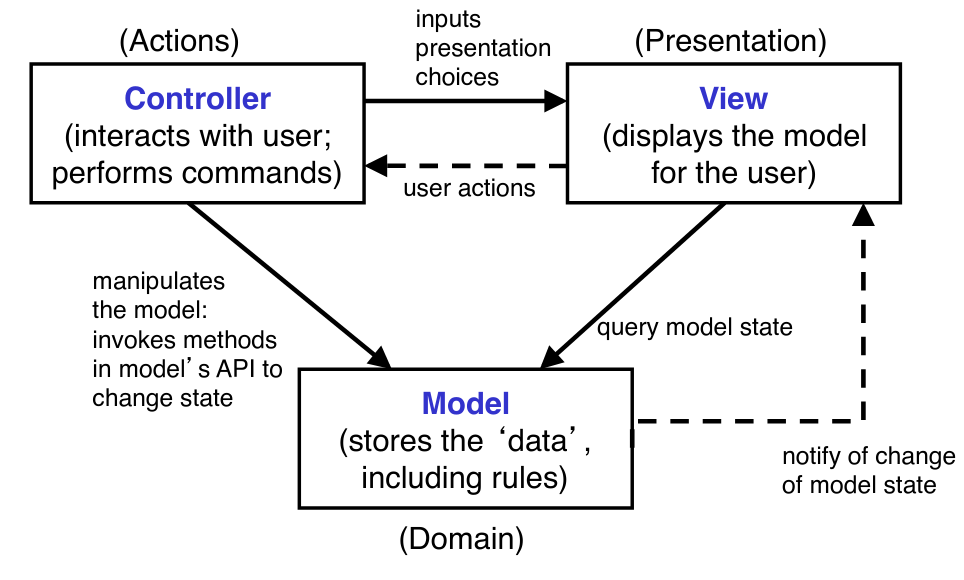
\includegraphics[scale=0.7]{MVC}
\end{center}
\section{Patterns vs Styles}
Architectural patterns are concerned with:
\begin{itemize}
	\item Defining the basic structure for an application
	\item Addressing a specific problem as well as the solution
\end{itemize}
Architectural styles are concerned with:
\begin{itemize}
	\item Families of software systems in terms of their structural organisation
	\item The forms of, and the interactions between, components, connectors and the context within which these exist
\end{itemize}



\end{document}